% !TeX root = RJwrapper.tex
\title{The \pkg{bdpar} Package: Big Data Pipelining Architecture for R}
\author{by Miguel Ferreiro-D\'iaz, Tom\'as R. Cotos-Y\'añez, Jos\'e R. M\'endez and David Ruano-Ord\'as}

\maketitle

\abstract{
In the last years, big data has become a useful paradigm for taking advantage of multiple sources to find relevant knowledge in real domains (such as the design of personalized marketing campaigns or helping to palliate the effects of several fatal diseases). Big data programming tools and methods have evolved over time from a MapReduce to a pipeline-based archetype. Concretely the use of pipelining schemes has become the most reliable way of processing and analyzing large amounts of data. To this end, this work introduces 
\pkg{bdpar}, a new highly customizable pipeline-based framework (using the OOP paradigm provided by \CRANpkg{R6} package) able to execute multiple preprocessing tasks over heterogeneous data sources. Moreover, to increase the flexibility and performance, \pkg{bdpar} provides helpful features such as (i) the definition of a novel object-based pipe operator (\code{\%>|\%}), (ii) the ability to easily design and deploy new (and customized) input data parsers, tasks, and pipelines, (iii) only-once execution which avoids the execution of previously processed information (instances), guaranteeing that only new both input data and pipelines are executed, (iv) the capability to perform serial or parallel operations according to the user needs, (v) the inclusion of a debugging mechanism which allows users to check the status of each instance (and find possible errors) throughout the process.
}

\section{Introduction}

Social networks and instant messaging applications have arguably become an essential part of the human experience. In fact, nowadays, more than 60\% of the population from industrialized countries use these mechanisms to communicate or share information. This phenomenon emerged due to (i) the declining costs of computers and storage systems by a factor of more than 200 \citep{D1}, (ii) an exponential increase in processing speed and computer hardware capabilities \citep{D2}, (iii) the emergence of high-throughput and fully-available communication networks \citep{D3}, and (iv) certain human needs such as keeping interconnected and having permanent access to the data \citep{D4}.

This scenario has promoted an exponential growth in the amount of data generated and stored in the last decade. Concretely, the latest reports from 2018 showed that around 2.16EB (exabytes) of data are created every day \citep{D5, D6}, and trends are showing that the growth of available information is four times higher than the world economy \citep{D6}. Indeed, 90\% of the total world data have been created in the last two years alone \citep{D7}. 

In addition to the availability of unlimited sources and tools to generate, exchange, and handle information, the lack of a standardized way of representing data has led to a massive increase in unstructured information. In fact, approximately 80\% of the existing data is unstructured \citep{D6, D7}. The data obtained from a single source are usually insufficient to carry out a suitable decision making-process. However, the ability to take advantage of the combination of data from multiple (and unstructured) sources requires the execution of preprocessing operations that guarantee a unified data format. The need for facilitating the management and exploitation of vast amounts of heterogeneous data (in terms of data types and formats) within a reasonable elapsed time and cost-effective manner led to the emergence of the Big Data era \citep{D8, D9}. 

Big Data is an abstract concept used to refer to the use of new programming paradigms able to handle large volumes of information and the execution of data mining tasks by taking advantage of parallel programming schemes over large computer clusters \citep{D10, D11}. In this context, MapReduce \citep{D12, D13} is the most popular programming model to develop, execute and deploy Big Data analyses on large clusters. However, its batch-processing nature forces uploading data to the system (cluster) every time is analyzed, even when the input data has been previously utilized. This requirement (i) makes this programming paradigm unsuitable when leading with real-time streaming sources and (ii) avoids achieving full use of the computational capabilities and resources since clusters are idle while the data is being loaded. In order to solve these limitations, the utilization of pipelining schemes for big data processing was recently introduced by \cite{D14}. This concept (extrapolated from the electronic domain) is focused on dividing the whole data analysis process into a set of computationally simple tasks \citep{D15} whereby the required information for each task is handled exclusively, which avoids the (pre)loading of unnecessary information. This advantage has prompted the emergence of multiple enterprises offering cloud pipeline-based data analysis services such as BDB Solutions for Big Data \citep{D16}, AWS Amazon Data Pipeline \citep{D17} or Google Cloud Dataflow \citep{D18}. These services allow users to build highly customized pipelines using a simple graphical interface, even if their technical skills are basic. Despite the great advantages of these services, their cloud-oriented nature causes customers to be reluctant to use them due to (i) the full control of the pipeline by the company offering the service, (ii) data privacy and security concerns (since information is executed in a foreign infrastructure), and (iii) the difficulty of assessing and calculating the cost of computational resources required to process data through the defined pipeline.

In order to cope with these problems, several customers decided to change the third-party cloud-based service to a proprietary solution by designing and implementing their own pipelining tools. Meanwhile, multiple open-source offline Big Data Pipeline frameworks emerged from the academic community to make this new paradigm available to everybody \citep{D14}. However, as can be observed from the list shown in \citep{D14}, despite the great number of available solutions, the majority are developed using Java language (>90\%) while only a few belong to the R ecosystems. Among these, two packages should be mentioned, \CRANpkg{repo} \citep{repo} and \CRANpkg{drake} \citep{drake}. The former one is a data-centered pipeline focused on solving bioinformatics data problems (specific-purpose application). Conversely, the latter is a generic pipeline tool that provides similar functionality to the GNU Make utility. As can be seen, despite both applications are focused on the same concept (pipelines), the target, implementation schema, and provided functionalities are quite divergent. In addition, we found some important issues that are not addressed by the actual pipelines tools such as (i) lack of a pure object-oriented (OO) implementation to facilitate the use and reduce the learning curve for people coming from object-oriented environments, (ii) the absence of an application based on the pipelining concept used by the well-known \CRANpkg{magrittr} package \citep{magrittr} (focused on UNIX pipes), (iii) the use of a black-box implementation which hampers users to easily trace and debug both code and the intermediate results.

This scenario motivated us to design and implement \pkg{bdpar}, a framework capable of unifying and preprocessing heterogeneous data through the development and execution of customizable pipelines. To this end, our package allows automatizing the management of a large amount of information by segmenting data into a sequence of simple and indivisible tasks (divide and conquer paradigm). Specifically, \pkg{bdpar} allows to (i) use or develop content extractors (such as SMS or email parsers), (ii) use and implement new preprocessing tasks (pipes), (iii) define customization pipelines (set of tasks) to achieve the desired (structured) output, (iv) visualize the intermediate results achieved by each instance after being processed by the tasks comprising the pipeline (white-box implementation), (v) prevent the re-execution of previously computed instances and tasks, and finally (vi) execute the pipeline following both a sequential or parallel paradigm.

This paper provides a full description of the main functionalities and resources of the \pkg{bdpar} package. The current version is 3.0.1, and an updated list (with the whole collection of resources) is available in the vignette document and the reference manual. The following section provides a complete description of the package structure and functionalities. Then, the use of the package is described, and finally, an illustrative case study is provided.

\section{Package structure and operation}

In order to exploit the main advantages and strengths of the object-oriented paradigm (such as maintainability, modularity, or inheritance), the \pkg{bdpar} package was fully developed using \code{R6} classes (package \CRANpkg{R6} \citep{R6}). Particularly, \pkg{bdpar} was implemented using R6 classes due to its high performance and ease of use when compared with other alternatives (such as S3 or S4) (\cite{D38, D39}). From an operational point of view, \code{R6} classes implemented in \pkg{bdpar} package are divided into three different categories: (i) data extraction functionalities; (ii) pipe-based operations; and finally (iii) \pkg{bdpar} framework configuration utilities.

The first category (data extraction methods) comprises all methods responsible for automatically detect the format and parse contents according to the inner structure of data gathered from input sources. The second category encapsulates the functionality of extracting features from the parsed information. By default, the \pkg{bdpar} framework provides a complete data preprocessing flow comprising 18 different tasks. Additionally, \pkg{bdpar} allows for the easy creation of new customized data flows by combining multiple tasks (object-based pipes). Finally, the third category of methods allows handling the configuration parameters needed for the proper operation of both the \pkg{bdpar} framework and some tasks using third-party functions (such as credentials for \CRANpkg{rtweet} \citep{D31} or \CRANpkg{tuber} \citep{D32}). 

In order to improve the readability of the code and facilitate the comprehension of each implemented class, a naming convention was adopted. Methods included in the data extraction category are labeled using \code{Extractor} as a prefix, followed by the type (or structure) of the input source (e.g., \code{ExtractorEml} and \code{ExtractorSms} methods are able to parse text contents from emails and SMS, respectively). Finally, pipe-based functionalities are named using the operation name followed by the suffix \code{Pipe} (e.g., \code{ToLowerPipe} and \code{FindHashtagPipe} are tasks designed to convert text characters to lowercase and detect Twitter hashtags from textual contents, respectively). 

As stated before, the \pkg{bdpar} framework is focused on designing, implementing, and deploying customized processing flows for the big data domain. In order to handle the information obtained from the input sources, the package uses a specific structure called \code{Instance}, which is responsible for storing the properties extracted by each pipe comprising the processing flow. To provide an insightful view of our \pkg{bdpar} framework, Figure~\ref{Figure1} provides a graphical representation of its inner operation, which is divided into two main stages: (i) data loading and (ii) pipeline executing.

\begin{figure}[H]
  \centering
  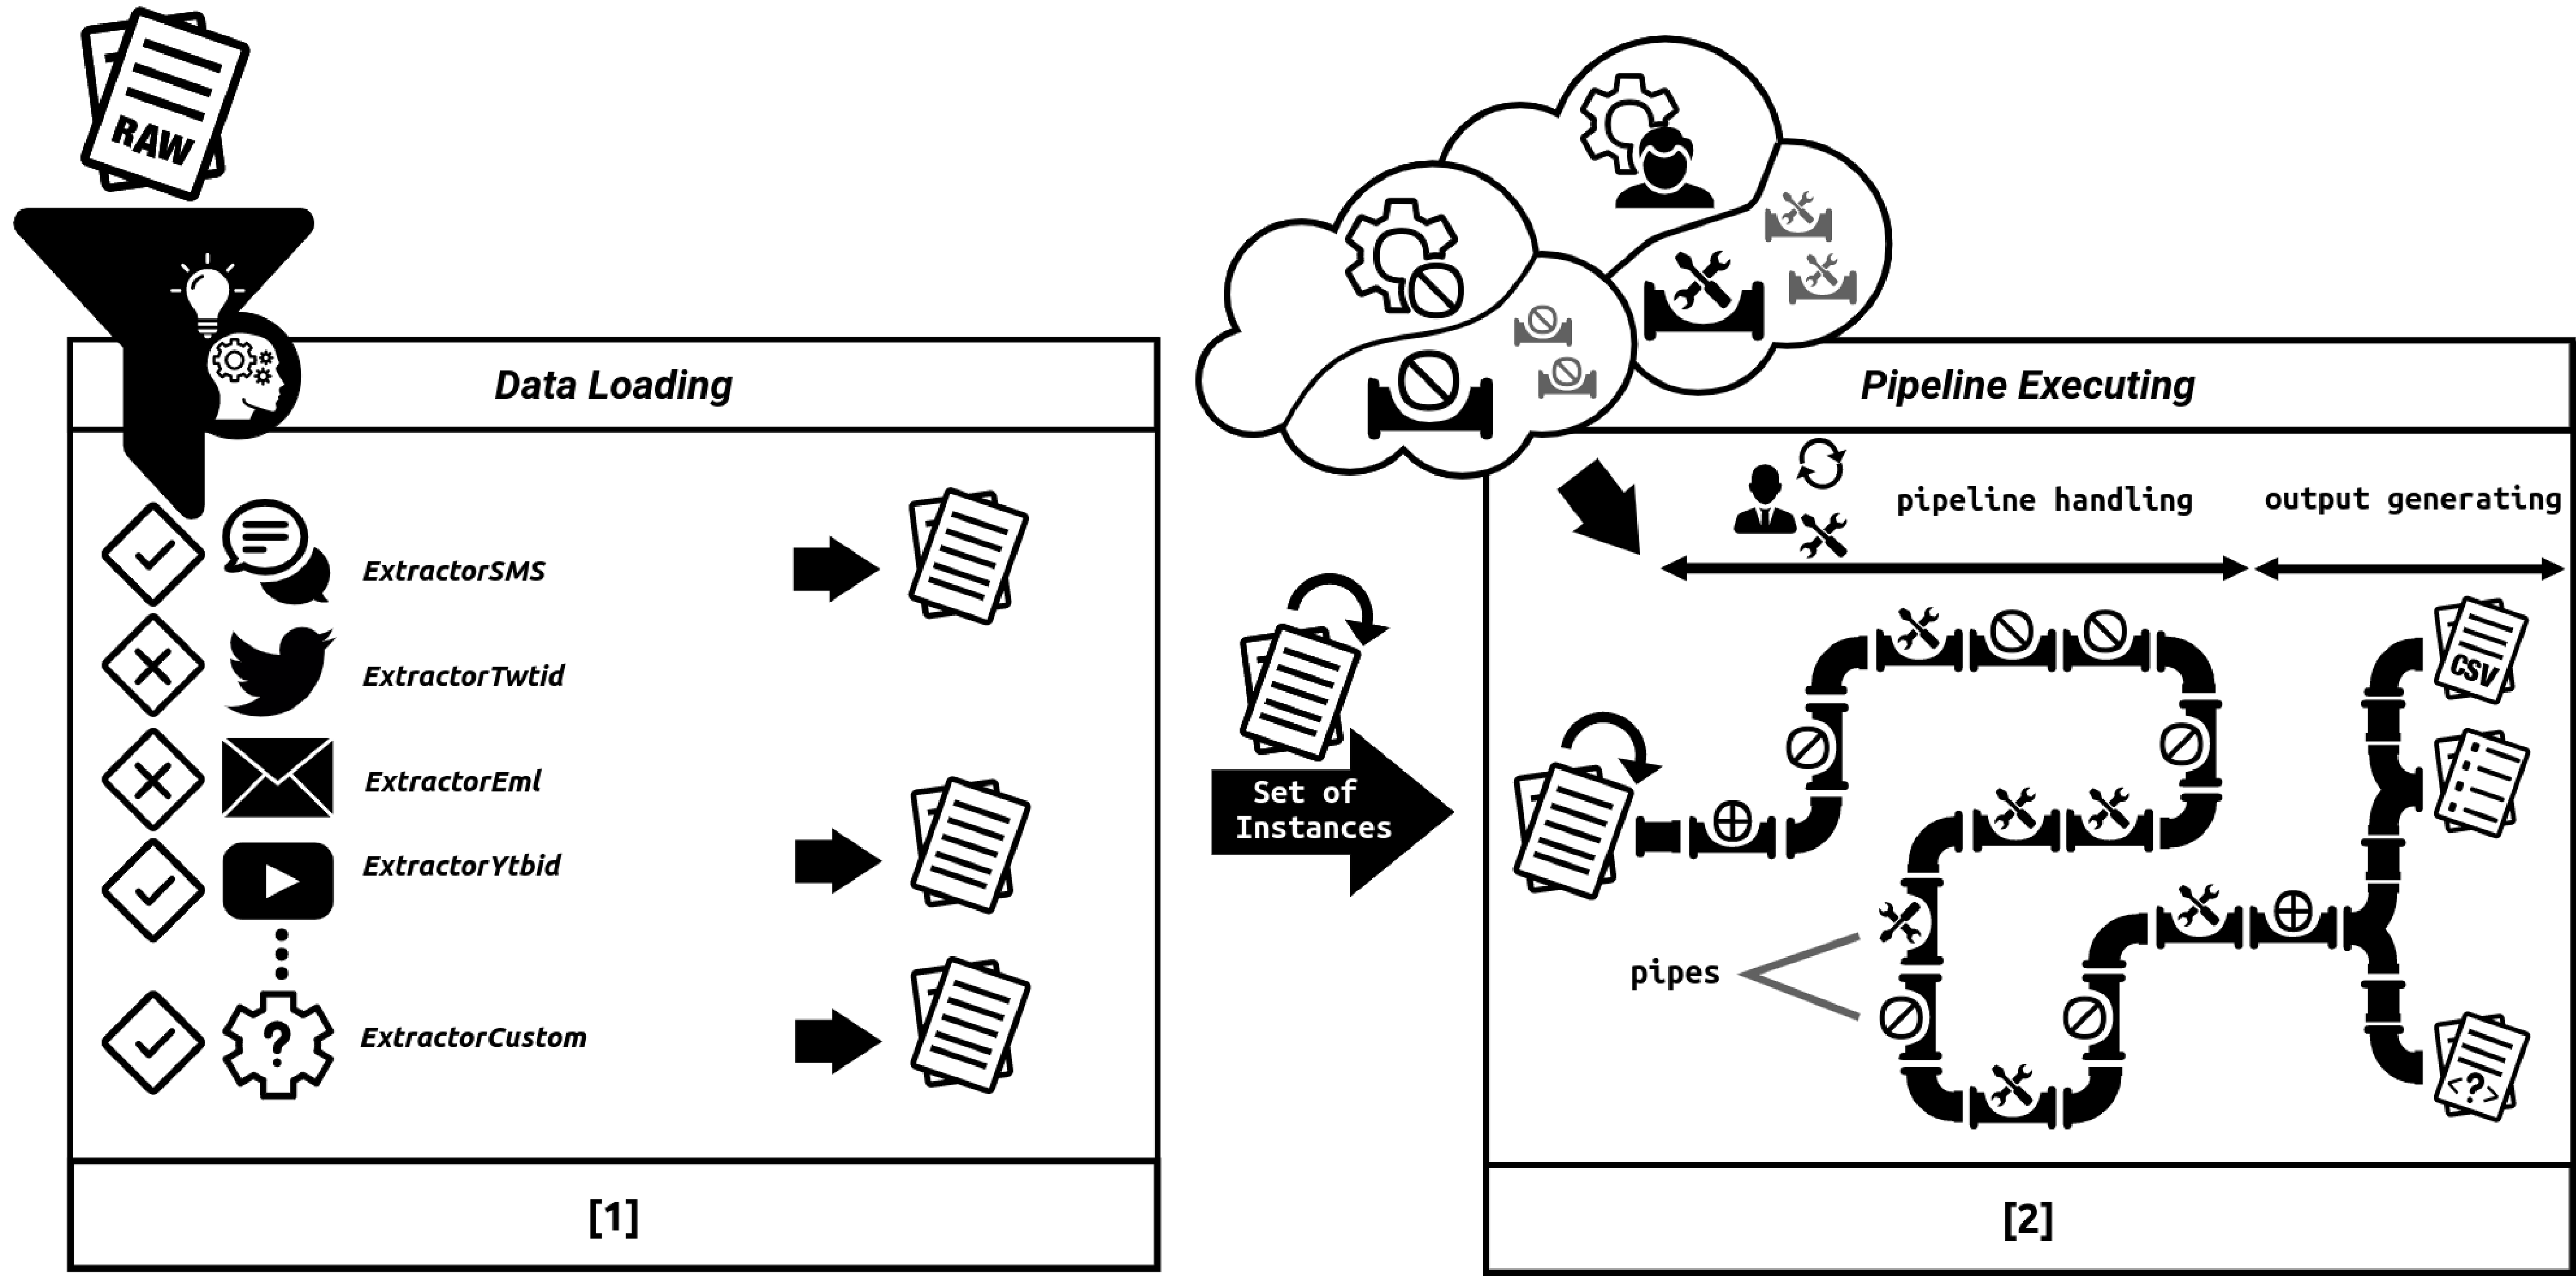
\includegraphics[width=\textwidth]{Figures/Figure1.pdf}
  \caption{Description of \pkg{bdpar} two-stage execution process. The first stage is responsible for loading the dataset, while the second stage is in charge of executing the pipes comprising the user-defined preprocessing tasks.}
  \label{Figure1}
\end{figure}

As shown in Figure~\ref{Figure1}, the first stage comprises the loading of the required extractors according to the type of input data. By default, \pkg{bdpar} provides four different types of extractors: (i) \code{ExtractorSMS} is able to extract the textual contents exchanged through Short Message Service (SMS); (ii) \code{ExtractorTwtid} is capable of obtaining the text from Twitter entries (tweets); (iii) \code{ExtractorEML} can be used to gathering raw content from the body of email messages, and finally (iv) \code{ExtractorYtbid} allows extracting the comments published on the YouTube platform. Additionally, to increase the compatibility of \pkg{bdpar} with other data formats, the framework allows for the easy design and deployment of new customized extractors (by using a simple OOP inheritance relation).

Once the content is successfully extracted from the raw sources, the second stage is automatically initiated by \pkg{bdpar}. This stage comprises the execution of two steps: (i) pipeline handling; and (ii) output generating. The former is in charge of performing unified data processing by executing a specific set of pipes (also named pipeline) over the previously extracted content. It should be noted that each pipe included in the pipeline is represented as an object (inherited from \code{GenericPipe} class) responsible for performing a specific operation (task) over the input data. The second step (called output generating) transforms the preprocessed data into a specific output format (e.g., into a CSV structure). Moreover, \pkg{bdpar} allows users to develop new specific output-generation methods to achieve the desired output.

As can be realized from the pipeline handling stage shown in Figure~\ref{Figure1}, the pipe-based structure provides great flexibility and versatility to users since it allows users to easily (i) modify existing pipelines by adding or removing pipes, (ii) develop new pipes implementing additional tasks, or (iii) design and deploy new customized pipelines. To assist users in the creation and deployment of new pipelines, \pkg{bdpar} provides a set of 18 combinable pipes implementing basic preprocessing tasks for text sources. As can be seen in Table~\ref{Table1}, tasks included in \pkg{bdpar} are divided into two different categories: (i) transformer tasks which are able to perform operations that successively alter the original content (such as lowercase conversion or emoticon finding), and (ii) maintainers which are responsible for executing operations that do not affect the current content (such as storing the extension of the input data). 

\begin{table}[H]
	\begin{tabularx}{\textwidth}{lccX}
		\toprule
		\multicolumn{1}{c}{Pipe name}	& Pipe type & \makecell{Name of computed\\property} & \multicolumn{1}{c}{Description} \\
		\toprule
		\code{GuessDatePipe} & Transformer & "date" & Obtains the date and time based on the type and structure of the input data. \\
	  	\code{File2Pipe} & Transformer & "source" & Obtains the source based on the type and structure of the input data.\\
		\code{FindUserNamePipe} & Transformer & "userName" & Detects and extracts usernames from textual sources.\\
		\code{FindHashtagPipe} & Transformer & "hashtag" & Detects and obtains hashtags from input data.\\
		\code{FindUrlPipe} & Transformer & "URLs" & Uses regular expressions to find URLs in text.\\ 
		FindEmoticonPipe & Transformer & "emoticon" & Identifies and extracts emoticons from textual sources.\\
		\code{FindEmojiPipe} & Transformer & "Emojis" & Transforms emojis to its textual representation.\\
		\code{GuessLanguagePipe} & Transformer & "language" & Tries to guess the language of a specific text.\\
		\code{ContractionPipe} & Transformer & "contractions" & Transforms previously detected contractions.\\
		\code{AbbreviationPipe} & Transformer & "abbreviation" & Expands detected abbreviations.\\
		\code{SlangPipe} & Transformer & "langpropname" & Identifies slang words to its corresponding formal speech.\\
		\code{ToLowerCasePipe} & Transformer & -- &  Converts the input source to lowercase characters.\\
		\code{InterjectionPipe} & Transformer & "interjection" & Detects and extracts interjections from textual sources.\\
		\code{StopWordPipe} & Transformer & "stopWord" & Recognizes and obtains stop words from textual sources.\\
		\code{TargetAssigningPipe} & Maintainer & "target" & Identifies the target class of the data.\\
		\code{StoreFileExtPipe} & Maintainer & "extension" & Guess the extension of the input data.\\
		\code{MeasureLengthPipe} & Maintainer & "length" & Computes the length of a given text.\\
		\code{TeeCSVPipe} & Maintainer & -- & Transforms the final result into a CSV format file.\\
		\bottomrule
	\end{tabularx}
	\caption{Pipes provided by \pkg{bdpar} framework.}
	\label{Table1}
\end{table}

Additionally, each pipe provides a property name field where the computed property will be stored. To increase flexibility, property names can be specified by users or leave it by default (see names described in Table~\ref{Table1}). Finally, pipes definition in Table~\ref{Table1} were sorted to match the execution order defined in the pipeline included by default in \pkg{bdpar} (named as \code{DefaultPipeline})

Moreover, to increase the reliability of the pipeline, \pkg{bdpar} allows defining the execution order of each task comprising the specified pipeline. During the definition of a pipeline, we should specifically take into account the possible interdependence between pipes (e.g., language-dependent tasks should be executed after \code{GuessLanguagePipe}). To solve this situation and ensure the proper creation and execution of the pipelining process, \pkg{bdpar} provides a pipe-orchestration system. This mechanism is automatically invoked when the pipeline is executed and traverses all tasks comprising the pipeline to evaluate two types of interdependencies: (i) always-before (or ‘a priori dependence’) and (ii) not-after (or ‘a posteriori dependence’). The first constraint is used when a specific pipe requires the previous execution of other tasks to ensure its proper operation (for instance, \code{AbbreviationPipe} needs to know the text language, so it should not be executed before \code{GuessLanguagePipe}). Conversely, the second type of restriction is used to indicate the tasks that cannot be started after the execution of the current one (for instance, the recognition of contractions should not be run after changing text characters to lowercase or removing punctuation marks). Both restrictions are automatically managed through the \code{checkCompatibility} method included in the \code{Instance} class. 

Furthermore, in order to ensure the proper execution of tasks implemented through \code{R6} classes within the pipeline, \pkg{bdpar} implements an object-oriented customized operator (denoted as \code{\%>|\%}) inspired by the implementation of the primitive forward-pipe operator (\code{\%>\%}) provided by the \pkg{magrittr} package \citep{magrittr}. Particularly, the execution of this new operator implies some inner operations such as (i) discarding an Instance (left-side operand) whenever an error occurs during the data processing flow, (ii) automatically manage pipes dependencies between pipes, (iii) simplifying the invocation of the associated pipe task (right-side operand) by hiding its explicit call, (iv) facilitate debugging issues by showing log messages with different levels of granularity, (v) the ability to display the intermediate computation results of each instance throughout the whole preprocessing flow and (vi) the capability to avoid the re-execution of previously processed pipelines. To this end, the operator transparently calls the \code{pipe} method defined in the pipe object. These functionalities allow improving the processing capabilities (in terms of speed, performance, and usability) of the application by preventing the problems derived from the (potential) existence of errors during the pipelining process and shorten pipelining definition by taking advantage of the customized operator capabilities. To increase the customization capabilities, \pkg{bdpar} allows easy development and deployment of new user-defined pipelines. To ensure full compatibility of new user-defined pipelines \pkg{bdpar} provides a reference class called \code{GenericPipeline}. Additionally, to simplify the use of the framework, \pkg{bdpar} provides a predefined pipeline (named \code{DefaultPipeline}) containing all the pipes included in Table~\ref{Table1}.

Finally, once all \code{Instance} objects are processed, the output generation stage starts. As can be seen from Figure~\ref{Figure1}, this stage is responsible for storing the results achieved after executing the pipeline process over each (valid) \code{Instance}. Although this stage allows the use of customized storage and output-representation methods (implemented by user), \pkg{bdpar} provides two methods able to (i) save the achieved output into an external CSV file (using \code{TeeCSVPipe} pipe) or (ii) internally store in memory a set of preprocessed \code{Instance} objects (default output).

In order to exemplify the structure and operation of an object-based pipeline in \pkg{bdpar}, we have included below a code snippet comprising 13 different text processing tasks (implemented as pipe objects). 

\begin{example}
instance %>|%
   TargetAssigningPipe$new() %>|% StoreFileExtPipe$new() %>|%
   GuessDatePipe$new() %>|% File2Pipe$new() %>|%
   MeasureLengthPipe$new("length_before_cleaning_text") %>|% 
   FindUrlPipe$new() %>|% FindEmojiPipe$new() %>|% GuessLanguagePipe$new() %>|%
   SlangPipe$new() %>|% ToLowerCasePipe$new() %>|% 
   InterjectionPipe$new() %>|% StopWordPipe$new() %>|%
   MeasureLengthPipe$new("length_after_cleaning_text") %>|% TeeCSVPipe$new()
\end{example}

To facilitate the understanding of the pipelining process, the code included above assumes that each input data has been successfully loaded and stored in an \code{Instance} object (denoted as \code{instance}). As can be seen from the code snippet, each \code{instance} is processed through all the tasks comprising this pipeline. Specifically, the first 13 ones perform different preprocessing operations over each \code{instance}, while the latest one stores the achieved results into a CSV file.

\section{Using \pkg{bdpar} package}

The package can be installed and attached as described in the code included below (please refer to the \file{README} file to access the latest and development versions).

\begin{example}
install.packages("bdpar")
library(bdpar)
\end{example}

Please note that the core functionalities of \pkg{bdpar} require the previous installation of six R packages (described in the \samp{Imports} field included in the \file{DESCRIPTION} file). In addition, some optional tasks (mainly belonging to specific data-processing pipes) used certain packages (indicated on the \samp{Suggest} field included in the \file{DESCRIPTION} file) and should also be installed in order to ensure its proper operation. It should be taken into account that in case of needing all the dependencies, the argument \code{dependencies = TRUE} should be included in the command \code{install.packages}.

\subsection{Executing \pkg{bdpar} framework}

In order to guarantee a high level of flexibility, \pkg{bdpar} can be easily executed by using two different ways (i) following an OOP paradigm or (ii) using a classical function call approach. Below is include a code snippet describing both scenarios.

\begin{example}
bdpar <- Bdpar$new()
bdpar$execute(path, extractors= ExtractorFactory$new(),
              pipeline= DefaultPipeline$new(), cache= TRUE, 
              verbose= FALSE, summary= FALSE)
\end{example}
a) Executing \pkg{bdpar} using OOP paradigm

\begin{example}
output <- line(path, extractors = ExtractorFactory$new(), 
               pipeline= DefaultPipeline$new(), cache= TRUE, 
               verbose= FALSE, summary= FALSE)
\end{example}
b) Executing \pkg{bdpar} following a function-based approach. 

As can be depicted, both execution methods require the same six arguments since \code{runPipeline} is a wrapper function which encapsulates \pkg{bdpar} execution using the OOP paradigm. The first argument is mandatory since it is used to specify the directory or file(s) path where the raw input data is located. The second parameter indicates the extractors required to parse the input sources. If not defined, \pkg{bdpar} automatically invokes the default \code{ExtractorFactory\$new()} object which initializes the four extractors provided by \pkg{bdpar} framework. Following, the third argument is used to determine the sequence of preprocessing tasks that should be executed (pipeline) to achieve the desired output (featured dataset). If the argument is not assigned, \pkg{bdpar} executes \code{DefaultPipeline\$new()} object which implements an error-safe pipeline comprised of 18 tasks described in Table~\ref{Table1}. The fourth one is used to enable (or disable) \pkg{bdpar} not-re-execution functionality (defined as \code{N-RE}). Particularly, this feature is able to detect which instances, tasks, and even pipelines were previously executed with a view to avoiding their re-execution. Moreover, the penultimate argument is used to indicate (if needed) the generation of a log output showing different levels of granularity (\code{DEBUG}, \code{INFO}, \code{WARN}, \code{ERROR}, \code{FATAL}). It should be noted that \code{DEBUG} level allows displaying the intermediate results achieved by each instance after being processed by the tasks comprising the pipeline. This is very useful to detect the location of possible errors. Finally, the latter argument allows showing (if needed) a detailed summary of all the operations and tasks performed during the pipeline execution.

\subsection{Developing new functionalities}

As previously stated, the design of the software architecture of \pkg{bdpar} is focused on facilitating the customization of any stage of the process (data loader and pipeline executor). Specifically, \pkg{bdpar} allows users to: (i) defining new types of input data parses, (ii) creating new pipes, and (iii) implementing and deploying new preprocessing tasks.

Regarding the first aspect, the development of new content parsers involves two stages: (i) the implementation of a customized extractor by overriding solely the methods of the \code{Instance} class that are necessary to load the input and (ii) the registration of the created extractor so it can be loaded by the \pkg{bdpar} framework. Two code fragments to detail the development and registration of a new customized parsers is included below.

\begin{example}
ExtractorImage <- R6::R6Class(
  classname = "ExtractorImage",
  inherit = Instance,
  public = list(
    initialize = function(path) {
      super$initialize(path)
    },
    obtainSource = function() {
      source <- imager::load.image(super$getPath())
      super$setSource(source)
      super$setData(source)
    } ) )
\end{example}
a) Implementation of new \code{ExtractorImage} parser.	

\begin{example}
extractors <- ExtractorFactory$new()
extractors$registerExtractor(extension= c("jpeg","png"), 
                             extractor= ExtractorImage)
\end{example}
b) Dynamic extractor registration operation in \pkg{bdpar}.

As can be seen, the first code snippet describes the formal structure of a new extractor. Particularly, \code{ExtractorImage} is able to load an image into an Instance object. To accomplish this task, the \code{obtainSource} method loads (by invoking \code{load.image()} method) an image from the file path received as a parameter of the class constructor (\code{super\$getPath()}). Then, the loaded image is stored in the source variable of the \code{Instance} superclass (by invoking \code{super\$setSource()} method) and is assigned to the data variable by calling to \code{super\$setData()} method. The data field is used to store the result of each task comprising the pipeline.

Moreover, the second fragment of code exemplifies the registration of the previously created extractor in \pkg{bdpar} framework. As can be depicted, this operation is performed by a simple call to the \code{registerExtractor} method included in \code{ExtractorFactory} class. Due to the one-to-one dependency between each extractor and the different input formats, \pkg{bdpar} requires the definition of a specific extension (or set of extensions) to discern which type of extractor should execute. Also, \code{ExtractorFactory} provides two additional methods (i) \code{getAllExtractors}, which shows all registered extractors in \pkg{bdpar} framework and (ii) \code{removeExtractor}, which deletes a specific data extractor. Finally, to avoid parsing errors, unsupported input contents by registered extractors are automatically ignored by \pkg{bdpar}.

For the creation and deployment of new preprocessing tasks, \pkg{bdpar} provides an abstract class named \code{GenericPipe}. This type of class is very common in OOP to ensure all subclasses (pipes) follow the same structure and implement the methods defined in the superclass (\code{GenericPipe}). Particularly, \code{GenericPipe} defines two main methods that should be included in each subclass: (i) \code{initialize} and (ii) \code{pipe}. The former includes three optional parameters that are \code{propertyName}, which refers to the specific name to the output value computed in the task, \code{alwaysBeforeDeps}, and \code{notAfterDeps}, which handles two types of dependencies between pipes ("always-before" and "not-after", respectively). Finally, the \code{pipe} method is used to implement the behavior of the new task. Below we include a code snippet exemplifying how to develop a basic image-preprocess pipeline. Concretely, we design three pipes: (i) \code{Image2Pipe} responsible for invoking the \code{obtainSource} method provided in the \code{ExtractorImage} parser, (ii) \code{ImageCroppingPipe} in charge of halving the image, and (iii) \code{ImageRotatePipe}, which rotates the image 30 degrees clockwise.

\begin{example}
Image2Pipe <- R6::R6Class(
  name = "Image2Pipe",
  inherit = GenericPipe,
  public = list(
    initialize = function(propertyName= "",
                          alwaysBeforeDeps= list(),
                          notAfterDeps= list()) {
      	    super$initialize(propertyName, alwaysBeforeDeps, notAfterDeps)
    },
    pipe = function(instance) {
      instance$obtainSource()
      instance
    } ) )

ImageCroppingPipe <- R6::R6Class(
  "ImageCroppingPipe",
  inherit = GenericPipe,
  public = list(
    initialize = function(propertyName= "",
                          alwaysBeforeDeps= list("Image2Pipe"),
                          notAfterDeps= list()) {
      	    super$initialize(propertyName, alwaysBeforeDeps, notAfterDeps)
    },
    pipe = function(instance) {
    data <- instance$getData()
    data <- imager::imsub(data, x > height/2)
    instance$setData(data)
      instance
    } ) )

ImageResizePipe <- R6::R6Class(
  "ImageResizePipe",
  inherit = GenericPipe,
  public = list(
    initialize = function(propertyName= "",
                          alwaysBeforeDeps= list("Image2Pipe"),
                          notAfterDeps= list()) {
      	    super$initialize(propertyName, alwaysBeforeDeps, notAfterDeps)
    },
    pipe = function(instance) {
    data <- instance$getData()
    data <- imager::imrotate(data, 30)
    instance$setData(data)
      instance
    } ) )
\end{example}

As can be seen, the \code{Image2Pipe} class stores the loaded image into a new instance. Following, \code{ImageCroppingPipe} and \code{ImageResizePipe} class apply different image manipulation functions (\code{imager::imsub}, \code{imager::imrotate}) to halve and rotate the images, respectively. Following the result, of each pipe is stored into a specific field of the \code{Instance} object (by calling the \code{instance\$setData()} method). To ensure proper operation of both tasks, image content should be previously loaded into an instance object (by invoking \code{Image2Pipe} associated task). To this end, a priori dependence with \code{Image2Pipe} has been defined in the \code{initialize} method of both pipes. As mentioned before, to facilitate the development and execution of pipes, dependencies between pipes are automatically managed by the object-oriented pipe operator (\%>|\%). Finally, in order to develop robust pipelines, \code{instance} objects should be invalidated when an error occurs, or the requirements are not satisfied (such as the storage of empty data or non-identification of textual language).

Finally, \pkg{bdpar} allows users to customize existing pipelines and develop new ones from scratch. In order to motivate the usage of \pkg{bdpar} regardless of user programming skills, the framework allows to manually or dynamically design new pipelines. The first method requires the creation of a new class (inheriting from \code{GenericPipeline}) which implements the \code{execute} method defined in the parent class. Moreover, to ensure proper management of (possible) execution errors (such as invalidated instances), a try-catch function should be included. Additionally, \pkg{bdpar} allows customizing the log messages (if needed) by calling the \code{bdpar.log()} function. Below we include an example showing how a customized pipeline is manually created. 

\begin{example*}
TestPipeline <- R6::R6Class(
  classname = "TestPipeline",
  inherit = GenericPipeline,
  public = list(
    initialize = function() {},
    execute = function(instance) {
      message("[TestPipeline][execute][Info] ", instance$getPath())
      tryCatch(
         instance %>|% Image2Pipe$new() %>|% 
             ImageCroppingPipe$new() %>|% ImageResizePipe$new(),
          error = function(e) {
               bdpar.log(message = paste0(instance$getPath()," :", paste(e)),
                 level= "ERROR",
                 className= class(self)[1],
                 methodName= "execute")
                 instance$invalidate()
        } )
      return(instance)
    } ) )
\end{example*}

On the other hand, the dynamic method allows the creation of custom pipelines by simply indicating a list containing the pipe objects to be used. To achieve a higher level of flexibility dynamic, the model provides two ways of defining pipelines: (i) during the object instantiation or (ii) by calling the \code{add} function. A simple example describing how the previous pipeline is created following the dynamic method is included below.

\begin{example}
pipeline <- DynamicPipeline$new(pipeline= list(Image2Pipe$new(),
                                               ImageCroppingPipe$new(), 
                                               ImageResizePipe$new()))
\end{example}
a) Pipeline definition during object instantiation.

\begin{example}
pipeline <- DynamicPipeline$new()
pipeline$add(list(Image2Pipe$new(), ImageCroppingPipe$new(), 
                  ImageResizePipe$new()))
\end{example}
b) Pipeline creation using the add method.

Additionally, the dynamic method provides six methods able to extend the pipeline customization capabilities: (i) \code{add(pipe, pos=NULL)}, which adds new pipe object(s) to the pipeline flow at a certain position (or at the end if not defined), (ii) \code{removeByPos(pos)}, which removes a pipe object at a given position, (iii) \code{removeByPipe(pipe.name)} responsible for erasing a \code{pipe} object by name, (iv) \code{removeAll()} capable of releasing all pipe objects from the pipeline, (v) \code{get()} returning a list containing the pipe objects comprising the pipeline, and finally, (vi) \code{print()} which displays the pipes comprised in the pipeline.

As can be realized from both methods, the manual definition of pipelines allows users to have greater control and insight over the pipeline (such as personalizing error-handling methods or the inclusion of new user-defined object-oriented pipeline operators). Conversely, the dynamic mode enables users to define optimal pipelines without expert knowledge of \code{R6} and OOP concepts.

\subsection{Managing \pkg{bdpar} configuration options}

\code{bdpar.Options} included in \pkg{bdpar} allows managing configuration parameters to customize the behavior of available tasks and indicate parameters needed for the proper operation of pipes and/or content extractors (such as path locations for slang dictionaries or credentials required by Twitter or Youtube APIs, respectively). Moreover, to easily search and access the configuration, \code{bdpar.Options} stores parameters following a key-value pair structure. As can be deducted, the key parameter is used to uniquely identify a configuration entry. In order to facilitate the management of configuration parameters, \code{bdpar.Options} provides four main methods: (i) \code{bdpar.Options\$add(key, value)}, which adds a new configuration entry, (ii) \code{bdpar.Options\$set(key, value)} used to modify the value of an existing configuration parameter, (iii) \code{bdpar.Options\$remove(key)}, which removes an entry matching a specific name, and finally, (iv) \code{bdpar.Options\$reset()} used to restore \code{bdpar.Options} to its initial state (default options). Table~\ref{Table2} describes the configuration options included in \pkg{bdpar}. 

\begin{table}[H]
	\begin{tabularx}{\textwidth}{cccl}
		\toprule
		Type & Key & \makecell{Assigned \\by default} & Description \\
 		\toprule
		API credentials	& \makecell[l]{twitter.consumer.key \\ twitter.consumer.secret \\ twitter.access.token \\ twitter.access.token.secret\\ \ \ \\youtube.app.id\\youtube.app.password} & 
											\makecell{ \  \ \\ x \\ \ \\ \ \\ x } & \makecell[l]{\ \\Set of keys need to\\connect to Twitter\\and Youtube API} \\
	  \midrule
		API cache & \makecell[l]{cache.youtube.path\\cache.twitter.path} & x & \makecell[l]{Path to temporary\\place extracted data}\\
		\midrule
		\makecell[l]{Pipe parameters} & \makecell[l]{teeCSVPipe.output.path} & \makecell{$\surd$} & \makecell[l]{Defines the out-\\put file path for\\\code{TeeCSVPipe}}\\
		\midrule
		\makecell[l]{Extractor options}	& \makecell[l]{extractorEML.mpaPartSelected} & \makecell{$\surd$} & \makecell[l]{Indicates the content-\\type to parse on multi-\\part emails}\\
		\midrule
		\makecell[l]{N-RE handler}	& \makecell[l]{cache.folder} & \makecell{$\surd$} & \makecell[l]{Indicates the path to\\store the intermediate\\results}\\
		\midrule
		\makecell[l]{Parallel settings}	& \makecell[l]{numCores} & \makecell{$\surd$} & \makecell[l]{Selects the number of\\cores used to execute\\the pipelines}\\
		\midrule
		\makecell[l]{Resource files} & \makecell[l]{resources.abbreviations.path \\ resources.contractions.path\\resources.interjections.path\\resources.slangs.path\\resources.stopwords.path} & \makecell{$\surd$} & \makecell[l]{Location for the dif-\\ferent language dic-\\tionaries (slang, con-\\tractions, $\ldots$)}\\
		\bottomrule
	\end{tabularx}
	\caption{Structure of \pkg{bdpar} configuration options.}
	\label{Table2}
\end{table}

As can be seen from Table~\ref{Table2}, configuration options are divided into seven categories: (i) API credentials, (ii) API cache, (iii) pipe parameters (iv) Extractor options, (v) instance cache handler, (vi) parallel settings, and (vii) resource files. It is important to take into account that values for API credentials are not provided by default due to the inexistence of publicly available access keys for both Youtube and Twitter (only for private use with prior approval). Following, the optional API cache configuration entries are responsible for designating temporal locations to store information obtained after executing the content extractors. Defining cache paths API ensures that duplicated sources are executed only once (avoids parsing duplicated inputs). 

Moreover, pipe parameters and extractor options allow specifying configuration values needed to guarantee the proper execution of pipes and extractors, respectively. Particularly, default "extractorEML.mpaPartSelected" entry allows defining which content-type (text/plain or text/html) should be extracted in multipart emails while "teeCSVPipe.output.path" indicates the location to store the CSV file generated by \code{TeeCSVPipe} pipe. 

In addition, the not-re-execution handler allows defining the path to store the information required for the proper operation of the not-re-execution functionality. Despite this, the feature is very useful to reduce both unnecessary computation costs and time consumption that requires extra storage space. Therefore, \pkg{bdpar} allows the deletion of the intermediate results by invoking the specific \code{bdpar.Options\$cleanCache()} method.

Following, parallel settings category is used to define the configuration values to handle parallelization in \pkg{bdpar}. Concretely, "numCores" entry allows defining the number of CPU cores to be used when a pipeline is executed. By default, \pkg{bdpar} is configured following a sequential paradigm (\code{numCores = 1}). Additionally, to ensure proper use of CPU resources \pkg{bdpar} provides a mechanism to verify whether the number of assigned CPU cores is compatible with the hardware specifications or not. If the assigned CPU cores are not valid, \pkg{bdpar} will be executed using the most optimal configuration according to the hardware specifications.

The last category comprises different dictionaries needed to perform multiple language-dependent operations (such as contraction detection or stopwords removal). Dictionaries provided by default ensure the compatibility of \pkg{bdpar} from 8 to 50 different languages (depending on the text-mining operation selected).

\section{A case study}

In order to illustrate the functionality of the \pkg{bdpar} package from a more realistic perspective, we developed a case study to show the most frequent words from a heterogeneous dataset collection (containing SMS and emails). The dataset comprises 20 emails (eml format) and 20 SMS in plain text from the nutritional and health domain. Moreover, to ensure straightforward reproducibility, (i) all the resources used are included in the package, and the pipeline provided by the package (\code{DefaultPipeline}) was selected to perform the content preprocessing flow, and (ii) resulting dataset was stored into a structured CSV file. Once the pipeline was executed, 18 new columns were generated from the outputs acquired after executing some pipeline tasks (labeled according to the property names described in Table~\ref{Table1}). For instance, the execution of \code{FindEmojiPipe} forces the creation (if not exists) of a new column (named "emojis") containing the emojis found for each instance (or blank if not found). 

To carry out the case of study, word frequencies were computed over the text content generated after executing the whole pipeline tasks (stored in the data column). Additionally, some previous text-cleaning operations were performed over the preprocessed text prior to executing the computation of the word frequencies (using word-cloud plots). Concretely, words were reduced to their stem form (stemDocument), punctuation marks were deleted, and numbers were removed (using the \CRANpkg{tm} package \citep{D37}). Finally, for comparison purposes, frequencies were calculated both individually and jointly (see Figures~\ref{Figure2} and ~\ref{Figure3})


\begin{example}
#Execute bdpar framework
bdpar::runPipeline(path= system.file(“example”, package= “bdpar”), 
                   cache= FALSE)
#Load CSV generated after executing bdpar
dataset <- read.csv(file= bdpar.Options$get("teeCSVPipe.output.path"), 
                    sep= ";", stringsAsFactors= FALSE )
                    
#Separate instances by type
sms <- dataset[dataset$extension == "tsms", ]
eml <- dataset[dataset$extension == "eml", ]
# Function to clean text and compute frequencies
word.frec <- function(data) {
  corpus <- tm::VCorpus(VectorSource(data))
  corpus <- tm::tm_map(corpus, removePunctuation)
  corpus <- tm::tm_map(corpus, removeNumbers)
  corpus <- tm::tm_map(corpus, stemDocument)
  sorted <- sort(rowSums(as.matrix(tm::TermDocumentMatrix(corpus))), 
                 decreasing = TRUE)
  return(data.frame(word = names(sorted), freq = sorted)) 
}
sms.words <- word.frec(sms$data)
eml.words <- word.frec(eml$data)
all.words <- word.frec(dataset$data)
# Wordcloud for sms and emails
par(mfrow=c(1,2))
wordcloud::wordcloud(words= sms.words$word, freq= sms.words$freq, 
                     min.freq= 1, max.words= 100, random.order= FALSE, 
                     rot.per= .5, colors= RColorBrewer::brewer.pal(8, "Dark2"))
wordcloud::wordcloud(words= eml.words$word, freq= eml.words$freq, 
                     min.freq= 1, max.words= 100, random.order= FALSE, 
                     rot.per= .5, colors= RColorBrewer::brewer.pal(8, "Dark2"))
par(mfrow=c(1,1))
#Wordcloud for all instances (sms and email)
wordcloud::wordcloud(words= dataset.words$word, freq= all.words$freq, 
                     min.freq= 1, max.words= 100, random.order= FALSE, 
                     rot.per= .5, colors= RColorBrewer::brewer.pal(8, "Dark2"))
\end{example}


Figure~\ref{Figure2} graphically represents the results achieved after performing an individualized analysis of each dataset (SMS and emails). Conversely, Figure~\ref{Figure3} represents the frequencies achieved when analyzing both datasets together. Observing Figure~\ref{Figure2}, we see that frequencies of words included in SMS messages are lower than those included in emails. This is mainly due to the limited length of SMS messages (up to 160 characters). Therefore, the word frequency in Figure~\ref{Figure3} has increased considerably, mainly owing to the joint evaluation of both datasets. 
\begin{figure}[H]
	\centering
	\begin{tabularx}{\textwidth}{XX}
		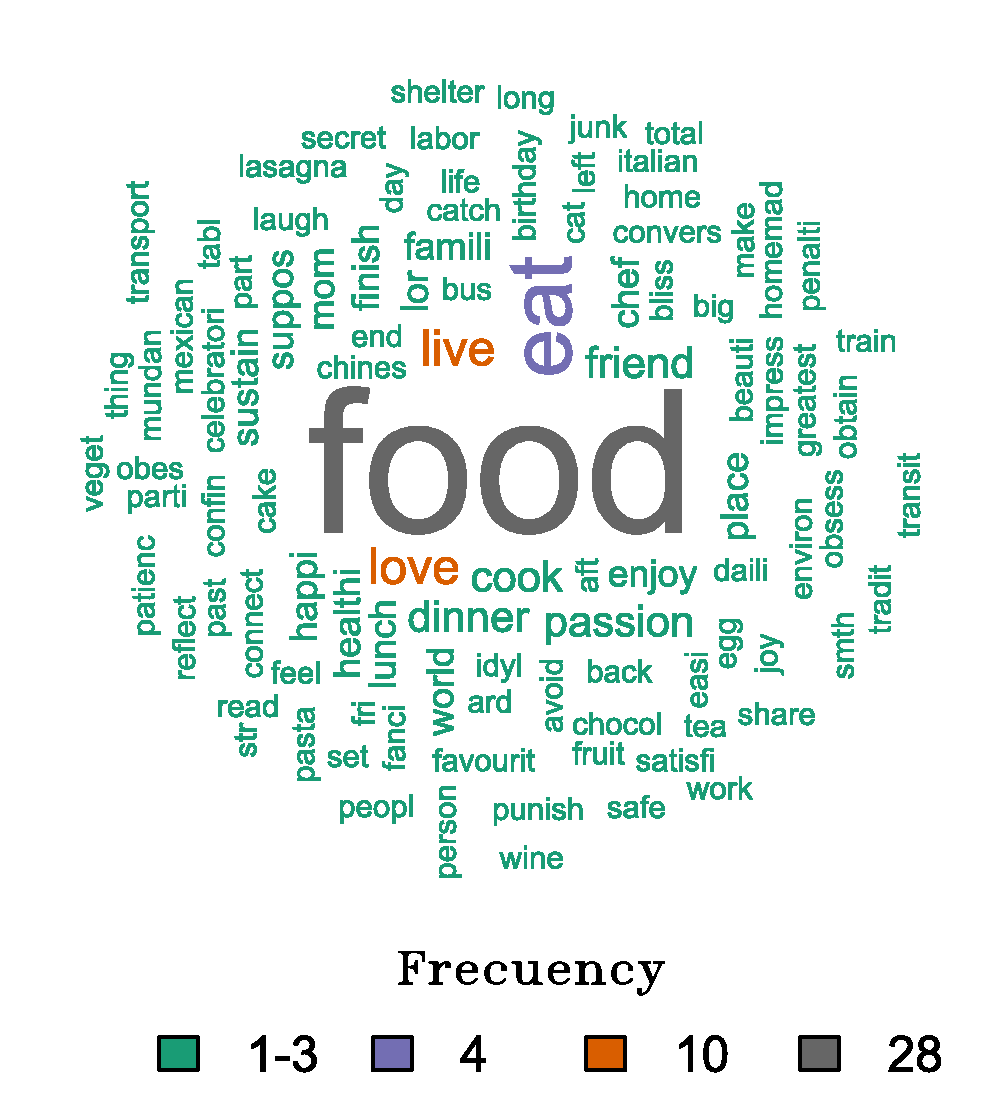
\includegraphics[width=.5\textwidth, height=.5\textwidth, keepaspectratio]{Figures/Figure2a.pdf}&
		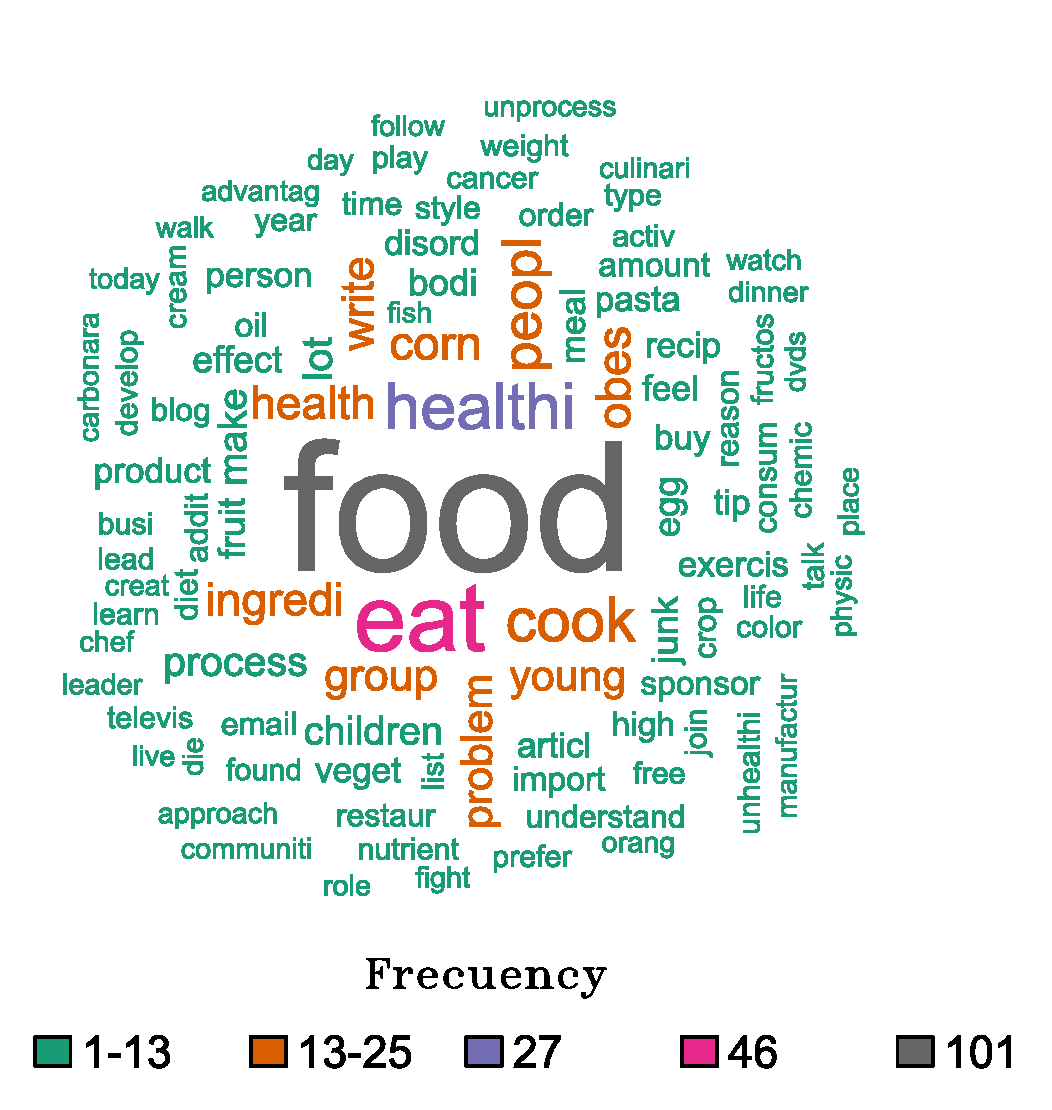
\includegraphics[width=.5\textwidth, height=.5\textwidth, keepaspectratio]{Figures/Figure2b.pdf}\\
	\end{tabularx}
	\caption{Wordcloud for SMS (left) and email (right).}
	\label{Figure2}
\end{figure}

\begin{figure}[H]
  \centering
  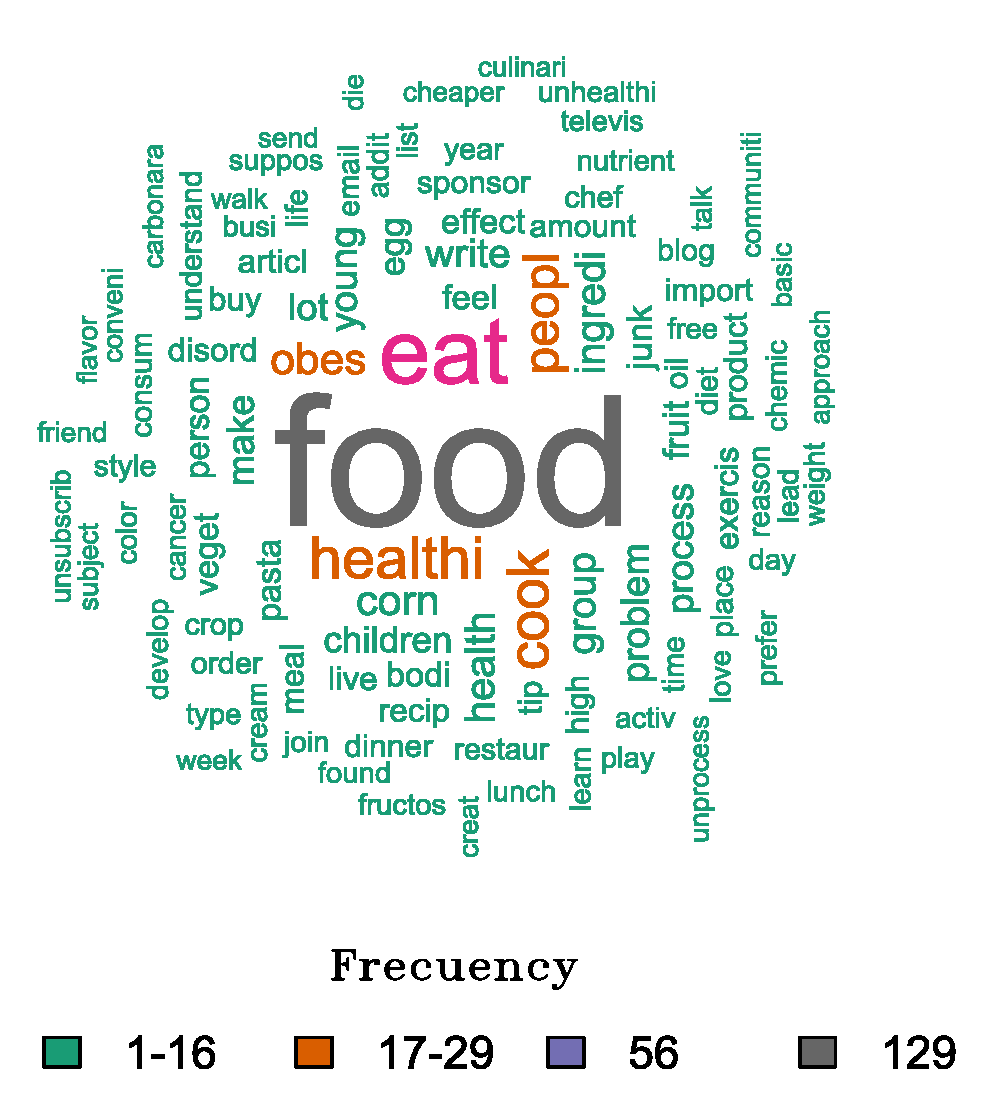
\includegraphics[width=.5\textwidth, height=.5\textwidth, keepaspectratio]{Figures/Figure3.pdf}
    \caption{Wordcloud for SMS and email jointly.}
  \label{Figure3}
\end{figure}

Keeping in mind the functionality provided by \pkg{bdpar} (demonstrated through the current case study), it is easy to deduce that the application of data mining techniques over unstructured data could be easily addressed by taking advantage of the functionality of our framework. Some big data operations that could be addressed by taking advantage of \pkg{bdpar} are the clustering of documents using token features, the classification of documents, or the retrieval of documents for specific queries.

\section{Conclusions and future work}
In this work, we introduced \pkg{bdpar}, a pipe-based R framework to facilitate the creation of unified datasets from heterogeneous sources. Our framework allows users to (i) define new content extractors (data parsers), (ii) develop and deploy new preprocessing tasks (pipes), and (iii) define and build customized interconnected task flows (pipelines). Additionally, to save computational resources and increase execution speed, \pkg{bdpar} provides an optimized pipe operator (noted as \code{\%>I\%}) capable of aborting the processing of an instance if an error was detected. Finally, a case study was developed to demonstrate the capability of the framework to preprocess and unify heterogeneous data into a single CSV file. 

Future work is focused on two main aspects: (i) the development of semantic-based tasks able to explode the semantic relationships between synsets and; (ii) the capability to represent using a graph-based visualization the pipes comprising each pipeline, and (iii) the analysis of textual polarity and sentiment analysis.

\section{Acknowledgements}
The work of Tomás R. Cotos-Yáñez has been partially supported by the projects IN2017-84658-C2-1-R and PID2020-118101GB-I00 of the Spanish Ministry of Industry.
David Ruano-Ordás has been supported by a post-doctoral fellowship from Xunta de Galicia (POSB-2021/024). Additionally, the work of Jos\'e R. M\'endez was partially funded by the project Semantic Knowledge Integration for Content-Based Spam Filtering (TIN2017-84658-C2-1-R) from the Spanish Ministry of Economy, Industry, and Competitiveness (SMEIC), State Research Agency (SRA) and the European Regional Development Fund (ERDF).
SING group thanks CITI (Centro de Investigación, Transferencia e Innovación) from the University of Vigo for hosting its IT infrastructure. Finally, we thank the reviewers for their deep appropriate suggestions to improve the quality of the manuscript.

\bibliography{ferreiro-cotos-mendez-ruano}

\address{Miguel Ferreiro-D\'iaz\\
	Department of Computer Science\\
	SING Research Group, University of Vigo, Spain\\
	CINBIO – Centro de Investigaciones Biom\'edicas, University of Vigo, Campus Universitario Lagoas-Marcosende, 36310 Vigo, Spain\\
	\email{miguel.ferreiro.diaz@uvigo.es}}

\address{Tomás R. Cotos-Yáñez\\
	Department of Statistics and Operations Research\\
	SiDOR Research Group, University of Vigo\\
	CINBIO – Centro de Investigaciones Biom\'edicas, University of Vigo, Campus Universitario Lagoas-Marcosende, 36310 Vigo, Spain\\
	ORCiD: 0000-0002-7732-6565\\
	\email{cotos@uvigo.es}}

\address{Jos\'e R. M\'endez\\
	Department of Computer Science\\
	SING Research Group, Galicia Sur Health Research Institute (IIS Galicia Sur), 
	SERGAS-UVIGO, Spain\\
	CINBIO – Centro de Investigaciones Biom\'edicas, University of Vigo, Campus Universitario Lagoas-Marcosende, 36310 Vigo, Spain\\
	ORCiD: 0000-0002-1935-4760\\
	\email{moncho.mendez@uvigo.es}}

\address{David Ruano-Ord\'as\\
	Department of Computer Science\\
	SING Research Group, Galicia Sur Health Research Institute (IIS Galicia Sur), 
	SERGAS-UVIGO, Spain\\
	CINBIO – Centro de Investigaciones Biom\'edicas, University of Vigo, Campus Universitario Lagoas-Marcosende, 36310 Vigo, Spain\\
	ORCiD: 0000-0002-6050-373X\\
	\email{drordas@uvigo.es}}